% Gemini theme
% https://github.com/anishathalye/gemini

\documentclass[final]{beamer}

% ====================
% Packages
% ====================

\usepackage[utf8]{inputenc}
\usepackage[T1]{fontenc}
\usepackage{lmodern}
\usepackage[orientation=portrait,size=a0]{beamerposter}
\usetheme{gemini}
\usecolortheme{gemini}
\usepackage{graphicx}
\usepackage{booktabs}
\usepackage{tikz}
\usepackage{pgfplots}
\usepackage{subcaption}   % For subfigure
\usepackage{mathtools}   % For mathclap
\pgfplotsset{compat=1.14}
\usepackage[table]{xcolor}
\usepackage[english]{babel}

% ====================
% Lengths
% ====================

% If you have N columns, choose \sepwidth and \colwidth such that
% (N+1)*\sepwidth + N*\colwidth = \paperwidth
\newlength{\sepwidth}
\newlength{\colwidth}
\setlength{\sepwidth}{0.025\paperwidth}
\setlength{\colwidth}{0.3\paperwidth}

\newcommand{\separatorcolumn}{\begin{column}{\sepwidth}\end{column}}

% ====================
% Title
% ====================

\title{AdamSLAM: the last mile of camera calibration with 3DGS}

\author{
    \begin{tabular}[t]{c@{\extracolsep{5em}}c}
  Matthieu GENDRIN, Stéphane PATEUX, Théo LADUNE & Xiaoran JIANG, Luce MORIN                    \\
  \textit{Orange Innovation}, France              & \textit{IETR}, France
    \end{tabular}
}

% ====================
% Footer (optional)
% ====================

\footercontent{
  \href{https://orange.com/}{https://orange.com/} \hfill
  ORASIS 2025, Le Croisic, France \hfill
  \href{mailto:matthieu.gendrin@orange.com}{matthieu.gendrin@orange.com}}
% (can be left out to remove footer)

% ====================
% Logo (optional)
% ====================

% use this to include logos on the left and/or right side of the header:
% \logoright{
%   \Large Paper ID: 132\hphantom{aaaaaa}
% }
% \logoright{\includegraphics[height=7cm]{logo1.pdf}}
\logoleft{
  
\includegraphics[height=5cm]{figures/orange_logo.png}
}

% ====================
% Body
% ====================

\begin{document}

% Longer legend line length
\pgfplotsset{
  compat=1.11,
  legend image code/.code={
  \draw[mark repeat=2,mark phase=2]
  plot coordinates {
  (0cm,0cm)
  (0.6cm,0cm)        %% default is (0.3cm,0cm)
  (1.2cm,0cm)         %% default is (0.6cm,0cm)
  };%
  }
  }

\begin{frame}[t]
\begin{columns}[t,totalwidth=2\colwidth]
\separatorcolumn

\begin{column}{1.5\colwidth}

  \begin{exampleblock}{Context \& contributions}

    3DGS (\inorange{3D Gaussian Splatting}) is a major breaktrough in novel view synthesis of volumetric scenes.
    It uses COLMAP \cite{schonberger2018robust} \inorange{camera calibration} as an input, which is not perfect.
    The quality of the camera calibration is of major importance for evaluating progresses in novel view synthesis, as a 1-pixel error on the calibration has a significant impact on the reconstruction quality. While there is no ground truth for real scenes, the quality of the calibration is assessed by the quality of the novel view synthesis. 

    \begin{figure}
        \centering
        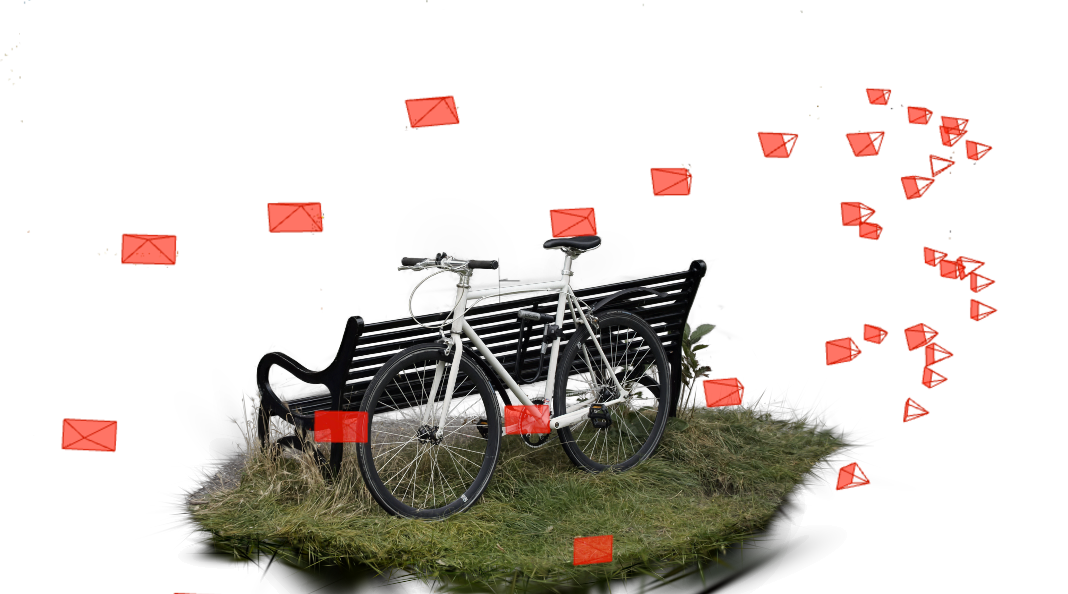
\includegraphics[height=15cm]{figures/pc_cams.png}
        \caption{Gaussian splatting model with cameras poses}
        \label{fig:pc_cams}
    \end{figure}
    
    \vspace*{1em}
    \textbf{Contributions: AdamSLAM}
    \begin{itemize}
      \item camera parameters fine-tuning by backpropagation of color loss on a 3DGS model
      \item average quality improvement of 0.4 dB PSNR 
    \end{itemize}
  \end{exampleblock}

  \begin{block}{AdamSLAM overview}
    During 3DGS reconstruction, the parameters of the cameras are trained by backpropagation of the loss color.
    \begin{figure}
    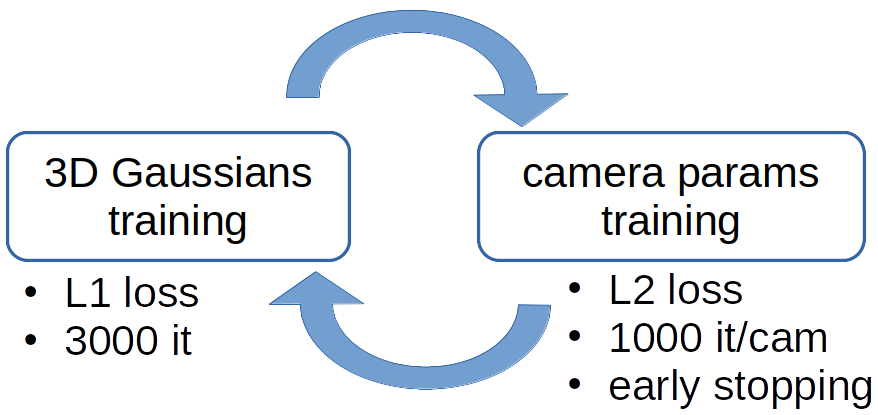
\includegraphics[width=30cm]{figures/method_scheduling.png}
    \end{figure}
  \end{block}
  
  \begin{block}{Back propagation simplification}
    Considering the impact of camera parameters mainly influences loss through the $u,v$ projection of the 
    points in image plan. Thus we simplify back propagation:
   \begin{align}
	\label{eq:2}
	\frac{\partial \mathcal{L}}{\partial p_j} = \sum_{i} \frac{\partial \mathcal{L}}{\partial uv_i^j} \frac{\partial uv_i^j}{\partial p_j}
    \end{align} 
  \end{block}

  \begin{block}{Early stopping}
    We propose a schedule by phase, with an early stopping mechanism to save compute time on cameras which do not benefit from fine-tuning. One camera is trained for at least 100 steps and maximum 1000 steps, a progress score being evaluated at every step. The training is interrupted when the progress score reaches a minimum threshold.
    This schedule \inorange{saves 20\%} of training time.

    \begin{figure}
    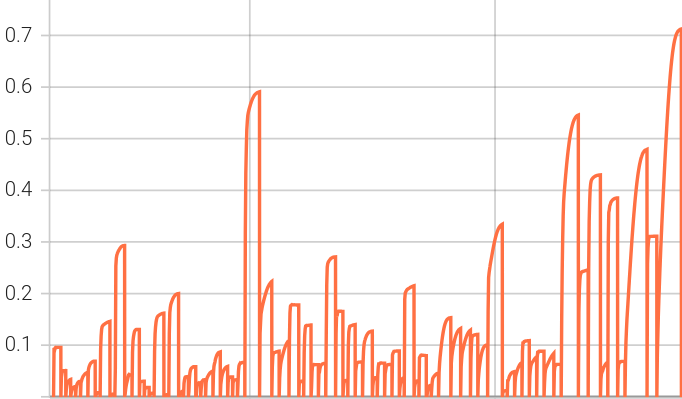
\includegraphics[height=10cm]{figures/delta_psnr_extract.png}
    \caption{PSNR improvement during cameras fine-tuning. Each phase concerns one camera. Y axis is the PSNR improvement of the current camera, x axis is the iteration.}\end{figure}
  \end{block}

\end{column}

\separatorcolumn

\begin{column}{1.5\colwidth}

\begin{block}{Reparameterization}
Consider the pinhole projection of the center of one gaussian whose position relative to the camera is $x,y,z$:
\begin{align}
	\label{eq:uv}
	(u, v) &= (\frac{f_x}{z} x, \frac{f_y}{z} y)
\end{align}
With $f_x,f_y$ the focal lengths of the camera, along $u,v$ axis.

Problem: $f_x, f_y$ and $z$ are \inorange{highly correlated} (getting closer to the scene is similar with zooming in with the camera).

Solution: $(z_c, \phi_x, \phi_y)$ are replaced by $(a, b, c)$, the coordinates in the referential defined by the eigen vectors of the Hessian matrix $\mathcal{H}$ of $\mathcal{L}(z_c,\phi_x,\phi_y)$.

The rational:
\begin{itemize}
    \item in the neighborhood of the local minimum $\frac{\partial \mathcal{L}}{\partial \theta} \approx \mathcal{H} \theta$
    \item $\frac{\partial \mathcal{L}}{\partial \theta_i} \approx \lambda_i \theta_i$ (with $\lambda_i$ the $i-th$ eigen value).
\end{itemize}

\begin{figure}
    \centering
    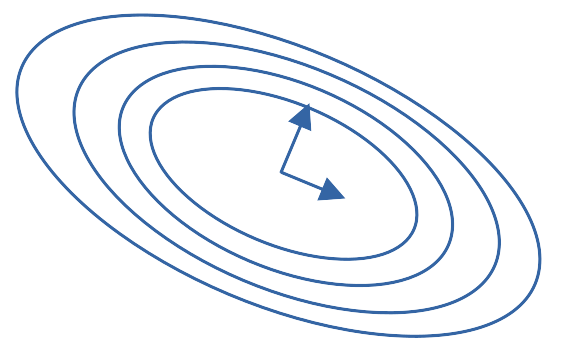
\includegraphics[width=0.5\linewidth]{figures/eigen_vectors.png}
    \caption{Illustration of level sets and eigen vectors.}
    \label{fig:eige_vectors}
\end{figure}

\end{block}

  \begin{block}{Results}

  Our test with the standard 3dgs algorithm show a \inorange{+0.4dB PSNR} improvement, with models that use
  \inorange{12\% less gaussians} than with the official camera calibration.

\begin{table}[h]
  \small
	\begin{center}
		{\rowcolors{2}{white}{blue}
		\begin{tabular}{|p{6cm}|c|c|}
			\hline
			scene & \shortstack{dataset calibration \\ PSNR [dB]} & \shortstack{ours \\ PSNR [dB]} \\
			\hline
			mip360 bicycle & 25.61 & \textbf{26.34} \\
			mip360 bonsai & 32.32 & \textbf{32.72} \\
			mip360 counter & 29.11 & \textbf{29.26} \\
			mip360 garden & 27.77 & \textbf{28.32} \\
			mip360 kitchen & \textbf{31.55} & 31.50 \\
			mip360 room & 31.72 & \textbf{31.94} \\
			mip360 stump & 26.90 & \textbf{27.28} \\
			T\&T Train & 22.12 & \textbf{22.61} \\
			T\&T Truck & 25.84 & \textbf{26.18} \\
			DB DrJohnson & 29.11 & \textbf{30.12} \\
			DB Playroom & 29.96 & \textbf{30.77} \\
			\hline
			Average & 28.36 & \textbf{28.82} \\
			\hline
			\end{tabular}
			}
			\caption{PSNR on the reference scenes as defined by 3DGS \cite{kerbl20233d}.
			Column "dataset calibration" lists results of training using the Colmap calibration provided with the datasets.
			Column "ours" lists results of training with the exact same code but our calibration.}
			\label{table:results}
		\end{center}
	\end{table}
	
  \end{block}

    \begin{figure}[h]
    	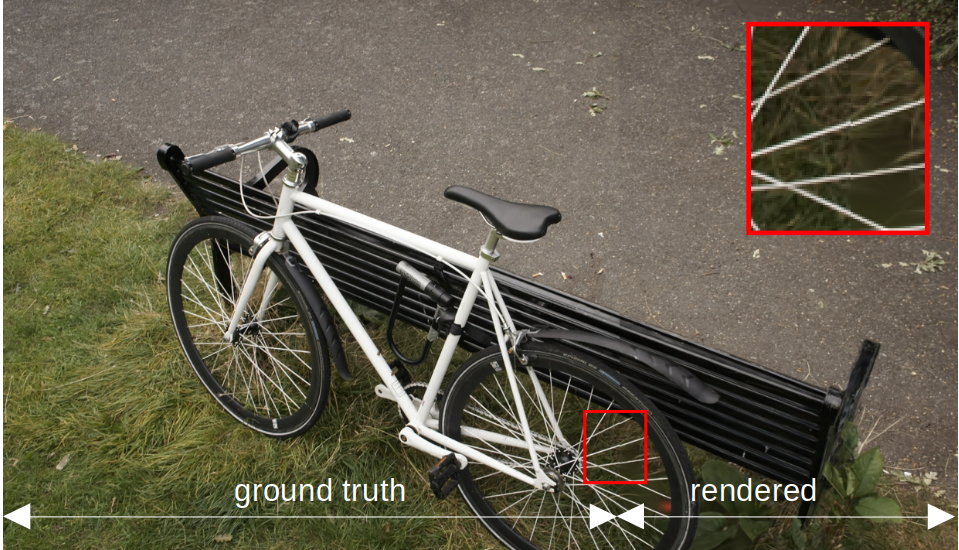
\includegraphics[height=8cm]{figures/bicycle-ref3.png}
    	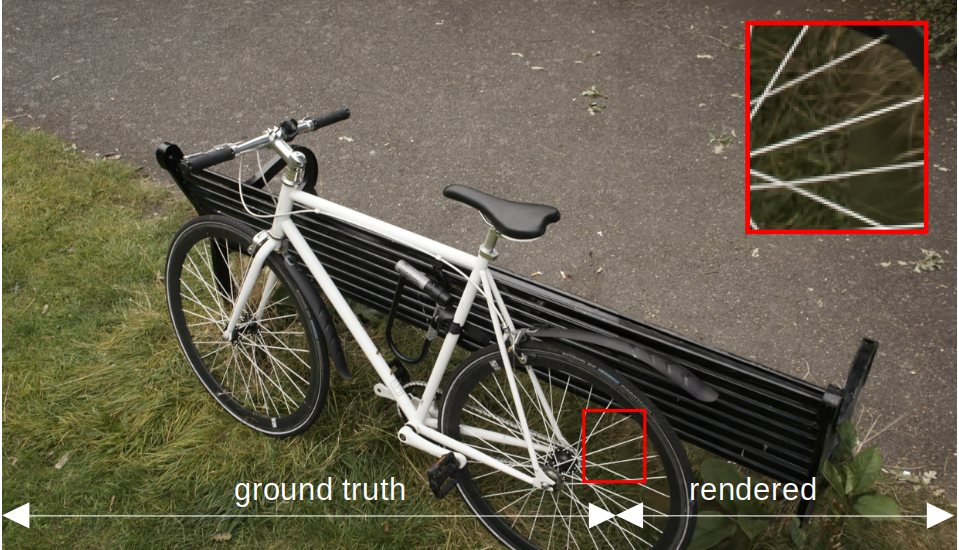
\includegraphics[height=8cm]{figures/bicycle-calib3.png}
    	\caption{Reference (top) vs ours (bottom) on bicycle view.}
    	\label{img:quali1}
    \end{figure}
    
  \begin{block}{References}
  % did not manage to import bibligraphy!
\begin{thebibliography}{1}

\bibliographystyle{plain}
\bibliography{
\bibitem{barron2022mip}
Jonathan~T Barron, Ben Mildenhall, Dor Verbin, Pratul~P Srinivasan, and Peter
  Hedman.
\newblock Mip-nerf 360: Unbounded anti-aliased neural radiance fields.
\newblock In {\em Proceedings of the IEEE/CVF conference on computer vision and
  pattern recognition}, pages 5470--5479, 2022.

\bibitem{HPPFDB18}
Peter Hedman, Julien Philip, True Price, Jan-Michael Frahm, George Drettakis,
  and Gabriel Brostow.
\newblock Deep blending for free-viewpoint image-based rendering.
\newblock {\em ACM Transactions on Graphics (SIGGRAPH Asia Conference
  Proceedings)}, 37(6), November 2018.

\bibitem{kerbl20233d}
Bernhard Kerbl, Georgios Kopanas, Thomas Leimk{\"u}hler, and George Drettakis.
\newblock 3d gaussian splatting for real-time radiance field rendering.
\newblock {\em ACM Trans. Graph.}, 42(4):139--1, 2023.

\bibitem{kingma2014adam}
Diederik~P Kingma and Jimmy Ba.
\newblock Adam: A method for stochastic optimization.
\newblock {\em arXiv preprint arXiv:1412.6980}, 2014.

\bibitem{knapitsch2017tanks}
Arno Knapitsch, Jaesik Park, Qian-Yi Zhou, and Vladlen Koltun.
\newblock Tanks and temples: Benchmarking large-scale scene reconstruction.
\newblock {\em ACM Transactions on Graphics (ToG)}, 36(4):1--13, 2017.

\bibitem{lindenberger2021pixel}
Philipp Lindenberger, Paul-Edouard Sarlin, Viktor Larsson, and Marc Pollefeys.
\newblock Pixel-perfect structure-from-motion with featuremetric refinement.
\newblock In {\em Proceedings of the IEEE/CVF international conference on
  computer vision}, pages 5987--5997, 2021.

\bibitem{schonberger2018robust}
Johannes~L Sch{\"o}nberger.
\newblock {\em Robust methods for accurate and efficient 3D modeling from
  unstructured imagery}.
\newblock PhD thesis, ETH Zurich, 2018.

\bibitem{Wang_2024_CVPR}
Shuzhe Wang, Vincent Leroy, Yohann Cabon, Boris Chidlovskii, and Jerome Revaud.
\newblock Dust3r: Geometric 3d vision made easy.
\newblock In {\em Proceedings of the IEEE/CVF Conference on Computer Vision and
  Pattern Recognition (CVPR)}, pages 20697--20709, June 2024.

\bibitem{ye2024gsplat}
Vickie Ye, Ruilong Li, Justin Kerr, Matias Turkulainen, Brent Yi, Zhuoyang Pan,
  Otto Seiskari, Jianbo Ye, Jeffrey Hu, Matthew Tancik, et~al.
\newblock gsplat: An open-source library for gaussian splatting.
\newblock {\em arXiv preprint arXiv:2409.06765}, 2024.
}
\end{thebibliography}

  
  \end{block}

\end{column}

\separatorcolumn
\end{columns}
\end{frame}
\end{document}
